
Le tableau de variations de la fonction $f$ est représenté ci dessous.

\begin{tikzpicture}
\tkzTabInit[lgt=1,espcl=2]{ $x$ / 0.7,$f $ / 1.4}
{ $-2$ , $-1$ ,1,3}
\tkzTabVar{+/$2$,-/$3$,+/$4$,-/$0$ }
\end{tikzpicture}

Qu'en penses tu ?
